
%%% Template originaly created by Karol Kozioł (mail@karol-koziol.net) and modified for ShareLaTeX use

\documentclass[a4paper,11pt]{article}

\usepackage[T1]{fontenc}
\usepackage[utf8]{inputenc}
\usepackage{graphicx}
\usepackage{xcolor}
\usepackage{graphicx} % Required to include images
\usepackage{caption}  % Optional, for better captions
\renewcommand\familydefault{\sfdefault}
\usepackage{tgheros}
\usepackage[defaultmono]{droidmono}
\usepackage{float} % in preamble
\usepackage{amsmath,amssymb,amsthm,textcomp}
\usepackage{enumerate}
\usepackage{multicol}
\usepackage{tikz}
\usepackage{url}
\usepackage{hyperref} 
\usepackage{geometry}
\geometry{left=25mm,right=25mm,%
bindingoffset=0mm, top=20mm,bottom=20mm}


\linespread{1.3}

\newcommand{\linia}{\rule{\linewidth}{0.5pt}}

% custom theorems if needed
\newtheoremstyle{mytheor}
    {1ex}{1ex}{\normalfont}{0pt}{\scshape}{.}{1ex}
    {{\thmname{#1 }}{\thmnumber{#2}}{\thmnote{ (#3)}}}

\theoremstyle{mytheor}
\newtheorem{defi}{Definition}

% my own titles
\makeatletter
\renewcommand{\maketitle}{
\begin{center}
\vspace{2ex}
{\huge \textsc{\@title}}
\vspace{1ex}
\\
\linia\\
\@author \hfill \@date
\vspace{4ex}
\end{center}
}
\makeatother
%%%

% custom footers and headers
\usepackage{fancyhdr}
\pagestyle{fancy}
\lhead{}
\chead{}
\rhead{}
\lfoot{Assignment \textnumero{} 5}
\cfoot{}
\rfoot{Page \thepage}
\renewcommand{\headrulewidth}{0pt}
\renewcommand{\footrulewidth}{0pt}
%

% code listing settings
\usepackage{listings}
\lstset{
    language=Python,
    basicstyle=\ttfamily\small,
    aboveskip={1.0\baselineskip},
    belowskip={1.0\baselineskip},
    columns=fixed,
    extendedchars=true,
    breaklines=true,
    tabsize=4,
    prebreak=\raisebox{0ex}[0ex][0ex]{\ensuremath{\hookleftarrow}},
    frame=lines,
    showtabs=false,
    showspaces=false,
    showstringspaces=false,
    keywordstyle=\color[rgb]{0.627,0.126,0.941},
    commentstyle=\color[rgb]{0.133,0.545,0.133},
    stringstyle=\color[rgb]{01,0,0},
    numbers=left,
    numberstyle=\small,
    stepnumber=1,
    numbersep=10pt,
    captionpos=t,
    escapeinside={\%*}{*)}
}

%%%----------%%%----------%%%----------%%%----------%%%

\begin{document}

\title{Programming Assignment \textnumero{} 2}

\author{Evangelia Panourgia, Athens University of Economics and Business University}

\date{27/03/2025}

\maketitle

\section*{Part I}
\subsection*{The python script for the first part.}

The provided Python script is an asynchronous Kafka producer designed to simulate real-time movie rating events. It uses the \texttt{Faker} library to generate synthetic user names and reads actual movie titles from a CSV file using \texttt{pandas}. Each generated user rates a randomly selected movie with a random rating between 1 and 10, along with a current timestamp. These events are serialized to JSON and sent to a Kafka topic named \texttt{"test"} using the \texttt{aiokafka} library. The process runs continuously, with each user producing one rating per minute, making it ideal for streaming applications such as those built with Apache Spark Structured Streaming. Additionally, the script appends a specific user name, ``Evangelia Panourgia'', to ensure consistent personal data inclusion for testing or filtering.


% code from http://rosettacode.org/wiki/Fibonacci_sequence#Python
\begin{lstlisting}[label={list:first},caption=python-kafka-example]
"""
Async Kafka Producer: Fake Movie Ratings Generator

Overview:
---------
This script continuously generates **fake movie rating events** and sends them to a Kafka topic ("test").
It simulates users rating random movies with timestamps, mimicking real-time data.

Components:
-----------
1. Faker: Generates fake human names.
2. Pandas: Loads real movie titles from a CSV file.
3. aiokafka: Asynchronous Kafka producer library.
4. Kafka: Acts as the message broker for event streaming.

Use Case:
---------
Run this script to simulate live rating data for a Spark Structured Streaming application to consume and process.
"""
import json
import asyncio
import random
from datetime import datetime

import pandas as pd
from faker import Faker
from aiokafka import AIOKafkaProducer

# Load movie titles
movies_df = pd.read_csv('data/movies.csv', header=None, names=["movie_title"])
movie_titles = movies_df['movie_title'].dropna().tolist()

# Generate names
fake = Faker()
names = [fake.name() for _ in range(10)]
names.append("Evangelia Panourgia") # add my own name

# Kafka settings
KAFKA_TOPIC = "test"
KAFKA_BOOTSTRAP_SERVERS = "localhost:29092"

# JSON serializer
def serializer(data):
    return json.dumps(data).encode()

# Producer logic
async def produce():
    producer = AIOKafkaProducer(
        bootstrap_servers=KAFKA_BOOTSTRAP_SERVERS,
        value_serializer=serializer,
        compression_type="gzip"
    )

    await producer.start()
    try:
        while True:
            for name in names:
                movie = random.choice(movie_titles)
                rating = random.randint(1, 10)
                timestamp = datetime.now().isoformat()

                message = {
                    "name": name,
                    "movie": movie,
                    "timestamp": timestamp,
                    "rating": rating
                }

                print(f"Sending: {message}")
                await producer.send(KAFKA_TOPIC, message)
                await asyncio.sleep(60) # One message per user per minute
    finally:
        await producer.stop()

# Run it (no deprecation warning)
if __name__ == "__main__":
    loop = asyncio.new_event_loop()
    asyncio.set_event_loop(loop)
    loop.run_until_complete(produce())


\end{lstlisting}

The image below depicts the output of kafka prodicer runing in the first terminal. 

\begin{figure}[h!]
    \centering
    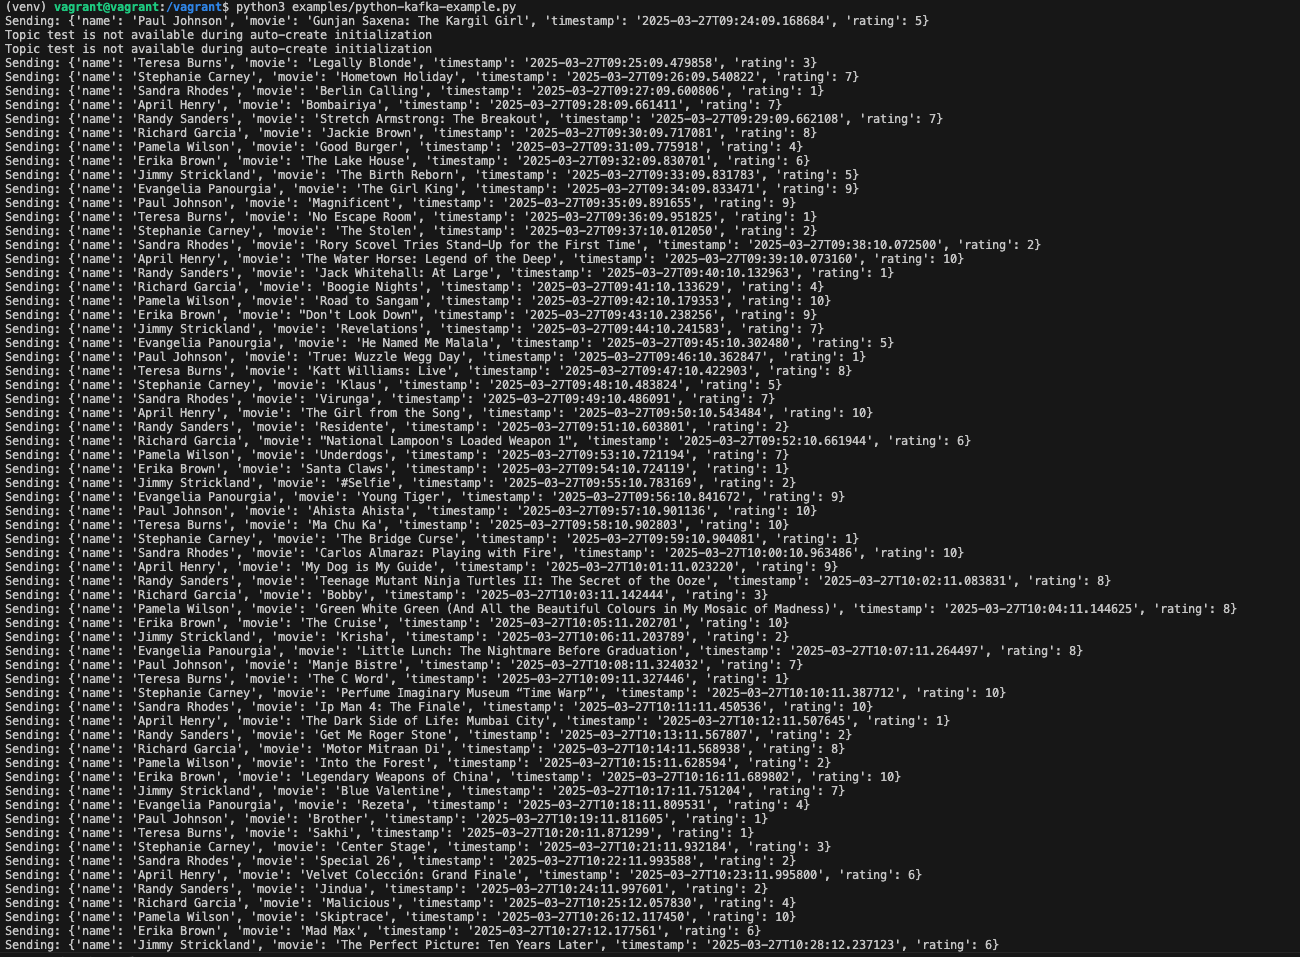
\includegraphics[width=0.8\textwidth]{1-kafka-data.png} % Replace with your image filename
    \caption{Terminal 1: Kafka Producer.}
    \label{fig:cassandra-sample}
\end{figure}


An additional modification was applied to the console script located in the \texttt{examples} directory, specifically to the file named \texttt{console-spark-streaming-example.py}. This adjustment was necessary to tailor the script to the project’s requirements and ensure compatibility with the streaming architecture.\\

The image below depicts the console output helping us to debug the kafka producer real-time data. It runs in another terminal. 

\begin{figure}[h!]
    \centering
    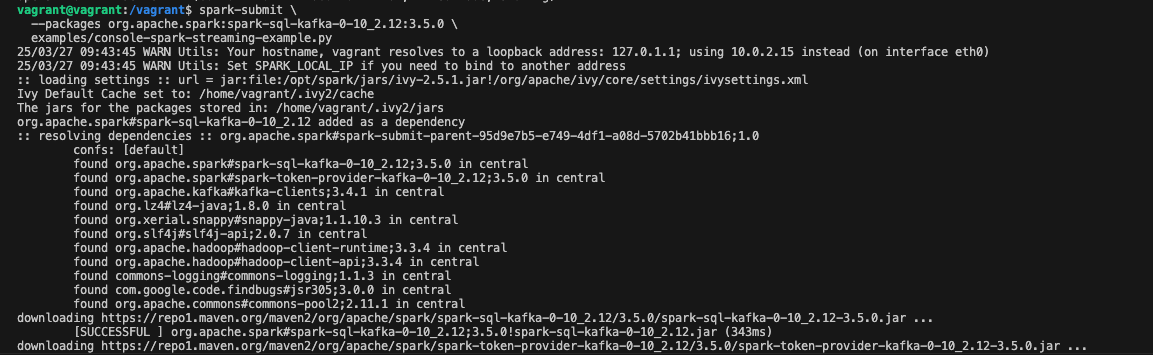
\includegraphics[width=0.8\textwidth]{2-console-debug-kafka.png} % Replace with your image filename
    \caption{Terminal 2: Console for Kafka Producer.}
    \label{fig:cassandra-sample}
\end{figure}

\section*{Part 2}
\subsection*{The pyspark script for the second part.}
This PySpark application establishes a real-time data pipeline that reads movie rating events from a Kafka topic, enriches them with metadata from a static Netflix dataset, and writes the processed results into a Cassandra database. The script defines two schemas: one for parsing JSON-encoded rating messages received from Kafka, and another for reading static metadata from a CSV file. It converts timestamps to proper \texttt{TimestampType}, and groups data by hourly buckets for time-based aggregations. Ratings are joined with metadata on the movie title to create an enriched DataFrame, which is then written to Cassandra using the \texttt{foreachBatch} method in micro-batch mode. This architecture enables structured streaming analysis and time-windowed queries for individual users and movies.\\

To improve performance and avoid repeated disk reads, the static Netflix metadata is cached in memory, ensuring it remains efficiently accessible during each micro-batch operation within the streaming query.\\


\begin{lstlisting}[label={list:second},caption=cassandra-spark-streaming-example.py.]
from pyspark.sql import SparkSession
from pyspark.sql.types import StructType, StructField, StringType, IntegerType, TimestampType
from pyspark.sql.functions import from_json, col, to_timestamp, date_format

# Schema for Kafka messages (movie ratings)
ratingSchema = StructType([
    StructField("name", StringType(), False),
    StructField("movie", StringType(), False),
    StructField("timestamp", StringType(), False),
    StructField("rating", IntegerType(), False)
])

# Schema for Netflix CSV
netflixSchema = StructType([
    StructField("show_id", StringType(), True),
    StructField("title", StringType(), False),
    StructField("director", StringType(), True),
    StructField("country", StringType(), True),
    StructField("release_year", StringType(), True),
    StructField("rating", StringType(), True),
    StructField("duration", StringType(), True)
])

# Initialize Spark session
spark = (
    SparkSession.builder
    .appName("MovieRatingStreamer")
    .config("spark.jars.packages", "org.apache.spark:spark-sql-kafka-0-10_2.12:3.5.0,com.datastax.spark:spark-cassandra-connector_2.12:3.4.1")
    .config("spark.cassandra.connection.host", "localhost")
    .getOrCreate()
)

spark.sparkContext.setLogLevel("ERROR")

# Read Netflix CSV with renamed rating column to avoid conflict with "rating" in Kafka schema
netflix_df = (
    spark.read.schema(netflixSchema)
         .option("header", True)
         .csv("data/netflix.csv")
         .withColumnRenamed("rating", "rating_category")  # Rename avoids conflict
         .cache()
)

# Read streaming data from Kafka
df = (
    spark.readStream.format("kafka")
         .option("kafka.bootstrap.servers", "localhost:29092")
         .option("subscribe", "test")
         .option("startingOffsets", "latest")
         .load()
)

# Parse JSON from Kafka messages
ratings_df = (
    df.selectExpr("CAST(value AS STRING)")
      .select(from_json(col("value"), ratingSchema).alias("data"))
      .select("data.*")
      .withColumn("timestamp", to_timestamp("timestamp"))  # Convert string timestamp to TimestampType
      .withColumn("hour_bucket", date_format("timestamp", "yyyy-MM-dd HH:00"))  # Grouping by hour
)

# Join ratings with static Netflix metadata
enriched_df = (
    ratings_df.join(netflix_df, ratings_df.movie == netflix_df.title, "left")
              .drop("title")
)

# Optional: Print schema for debugging (can be removed later)
enriched_df.printSchema()

# Define Cassandra write logic
def writeToCassandra(writeDF, _):
    (
        writeDF.select(
            "name", "movie", "timestamp", "rating", "hour_bucket",
            "show_id", "director", "country", "release_year", "rating_category", "duration"
        )
        .write
        .format("org.apache.spark.sql.cassandra")
        .mode('append')
        .options(table="movie_ratings", keyspace="netflix_ks")
        .save()
    )

# Write to Cassandra in a streaming loop
result = None
while result is None:
    try:
        result = (
            enriched_df.writeStream
                .foreachBatch(writeToCassandra)
                .outputMode("update")
                .option("checkpointLocation", "/tmp/checkpoints/movie")
                .trigger(processingTime="30 seconds")
                .start()
                .awaitTermination()
        )
    except Exception as e:
        print(f"Streaming error: {e}")
\end{lstlisting}

\subsection*{Details about your Cassandra data model.}

The Cassandra data model was carefully designed to optimize query performance for the specific requirement of aggregating movie ratings by user and hour. The primary key is composed of a composite partition key \texttt{(name, hour\_bucket)}, ensuring that all ratings provided by a specific user within a given hour are stored in the same partition. This design eliminates the need for inefficient filtering operations and allows for fast, targeted queries such as retrieving all movies rated by a user during a specific hour or calculating the average rating and duration of those movies. The clustering columns \texttt{(timestamp, movie)} further organize the data chronologically within each partition, enabling efficient range queries and ordered retrieval. Crucially, the fields \texttt{rating} and \texttt{duration} are stored as integers, allowing native support for aggregation functions like \texttt{AVG()}, which would not be possible with text fields. Overall, this schema supports the core analytical tasks required by the application while adhering to Cassandra’s best practices for scalability and performance.

\begin{lstlisting}[language=SQL,caption={Cassandra schema for movie ratings},label={lst:cassandra-schema}]
CREATE KEYSPACE IF NOT EXISTS netflix_ks
WITH replication = {'class': 'SimpleStrategy', 'replication_factor': 1};

CREATE TABLE IF NOT EXISTS netflix_ks.movie_ratings (
    name text,
    hour_bucket text,
    timestamp timestamp,
    movie text,
    rating int,
    show_id text,
    director text,
    country text,
    release_year int,         -- changed from text : int
    rating_category text,
    duration int,             -- changed from text : int
    PRIMARY KEY ((name, hour_bucket), timestamp, movie)
);
\end{lstlisting}

\begin{figure}[h!]
    \centering
    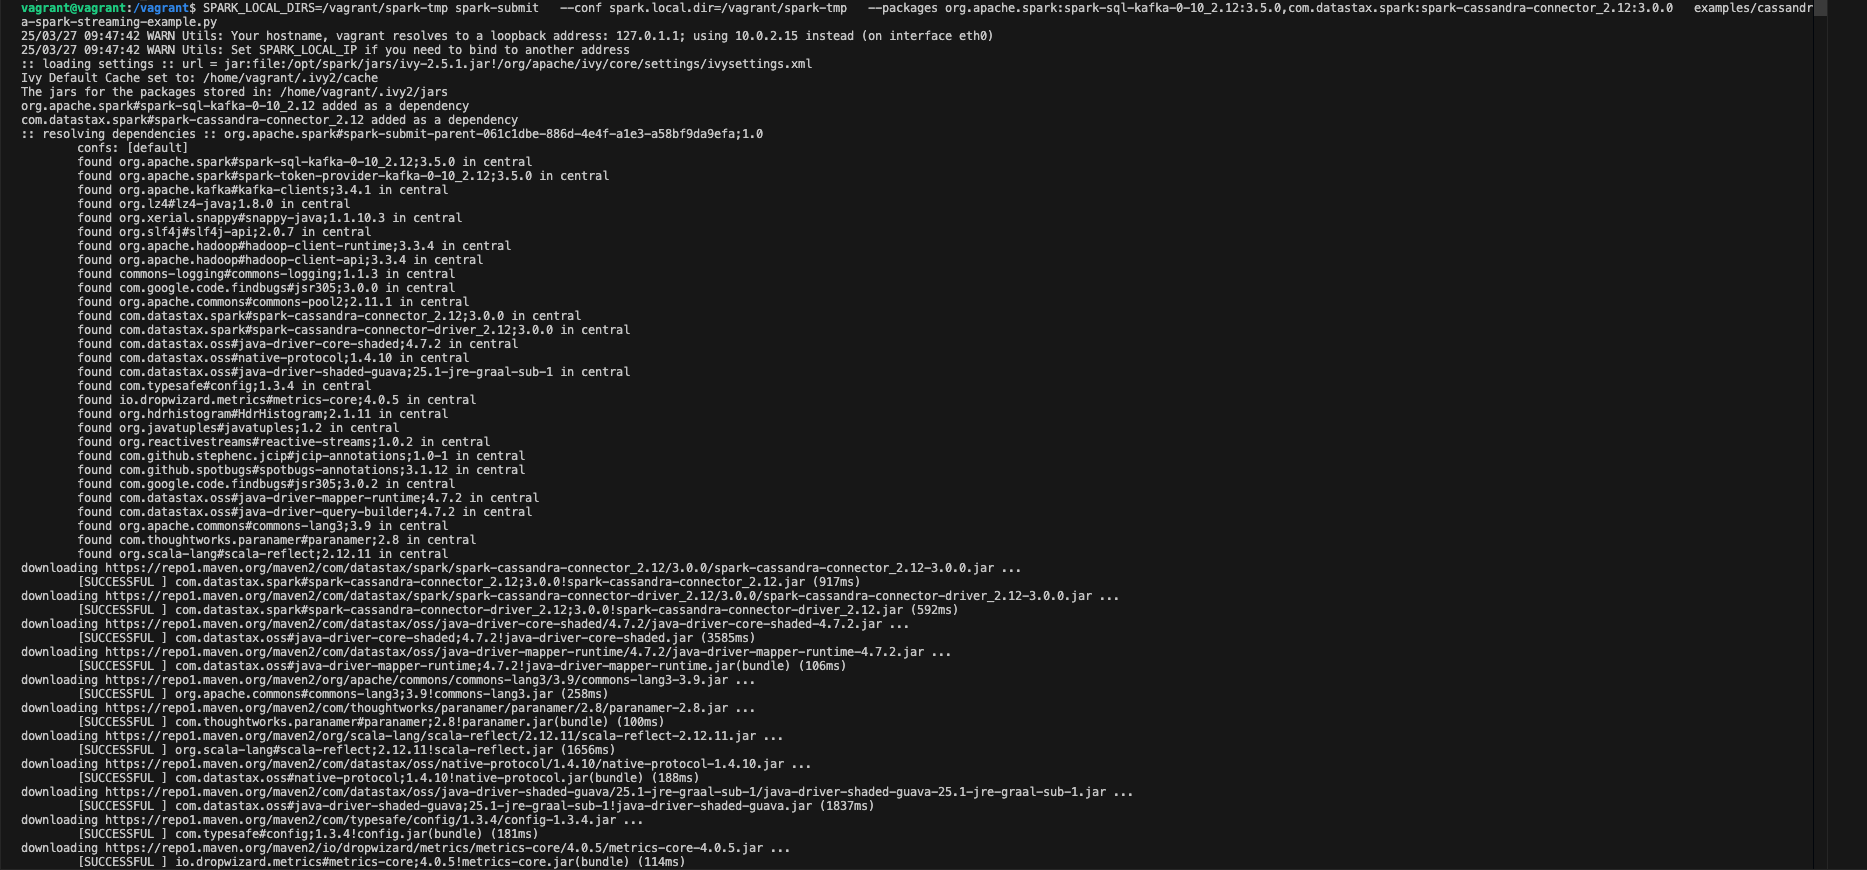
\includegraphics[width=0.8\textwidth]{4-spark-preprocess.png} % Replace with your image filename
    \caption{Terminal 3: Spark pre-process, enrich with metadata..}
    \label{fig:cassandra-sample}
\end{figure}

\subsection*{A sample of persisted lines (around 50) of your Cassandra table.}

To inspect the data stored in the \texttt{movie\_ratings} table of the \texttt{netflix\_ks} keyspace, we can use the \texttt{cqlsh} shell interface provided by Apache Cassandra. The following query retrieves approximately 50 rows that were previously persisted by the streaming pipeline:

\begin{verbatim}
SELECT * FROM netflix_ks.movie_ratings LIMIT 50;
\end{verbatim}

This query provides a representative snapshot of the data ingested into Cassandra, including key fields such as \texttt{name}, \texttt{movie}, \texttt{timestamp}, \texttt{rating}, and \texttt{duration}. Analyzing these records ensures data integrity, validates the correctness of the ingestion pipeline, and confirms that the schema design supports the desired querying capabilities.

\begin{figure}[h]
    \centering
    \includegraphics[width=0.8\textwidth]{5-sample-50.png} % Replace with your image filename
    \caption{A sample output of the Cassandra table with 50 persisted entries.}
    \label{fig:cassandra-sample}
\end{figure}

\subsection*{Two CQL queries and their results in your database about your own name and a particular
hour that generate the average runtime of the movies that you’ve rated during this hour, and
the names of the movies, respectively.}

To support time-based analytics in our Cassandra data model, we designed the schema to partition data by \texttt{name} and \texttt{hour\_bucket}, allowing efficient access to all ratings a specific user made during a given hour. The first query retrieves the titles of movies rated by the user \textit{Evangelia Panourgia} during the hour of \texttt{2025-03-27 09:00} using a direct lookup on the partition key. The second query, which includes the \texttt{ALLOW FILTERING} clause, calculates the average duration of those rated movies within the same hour. While Cassandra does not natively support aggregations without filtering, our schema minimizes performance issues by narrowing queries to a specific partition, ensuring practical execution even with the filtering clause.


\begin{figure}[H]
    \centering
    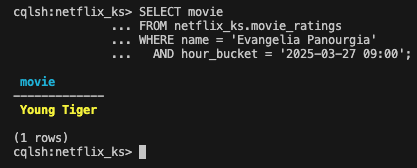
\includegraphics[width=0.8\textwidth]{q1.png} % Replace with your image filename
    \caption{ Names of the movies you rated during a particular hour
SELECT movie.}
    \label{fig:cassandra-sample}
\end{figure}


\begin{figure}[H]
    \centering
    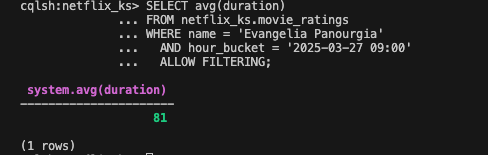
\includegraphics[width=0.8\textwidth]{q2.png} % Replace with your image filename
    \caption{Average duration of the movies you rated during the same hour
SELECT avg(duration).}
    \label{fig:cassandra-sample}
\end{figure}

Furthermore, after allowing the real-time streaming process to run for an additional hour, we re-executed the following queries—this time updating the hour\_bucket value from 09:00 to 10:00 to reflect the new time window.\\

\begin{figure}[H]
    \centering
    \includegraphics[width=0.8\textwidth]{q2-new.png} % Replace with your image filename
    \caption{ Names of the movies you rated during a particular hour
SELECT movie.}
    \label{fig:cassandra-sample}
\end{figure}


\begin{figure}[H]
    \centering
    \includegraphics[width=0.8\textwidth]{new.png} % Replace with your image filename
    \caption{Average duration of the movies you rated during the same hour
SELECT avg(duration).}
    \label{fig:cassandra-sample}
\end{figure}

Note: It is not necessary to explicitly include conditions such as IS NOT NULL in the CQL queries, as Cassandra automatically excludes null values from aggregation functions like AVG(). Therefore, rows with missing values for the targeted column are implicitly ignored during computation.\\

\section*{Hosted on GitHub Repository - Deploy Instructions.}
The complete implementation of this project is hosted on GitHub and is publicly accessible at \url{https://github.com/e-panourgia/large-data-kafka-cassandra}. The repository contains all necessary components, including Kafka producers, Spark Structured Streaming jobs, and Cassandra schemas. To execute the project, clone the repository using \texttt{git clone https://github.com/e-panourgia/large-data-kafka-cassandra}, then follow the instructions in the README file to set up Docker containers, start Kafka and Cassandra services, and run the streaming application using \texttt{spark-submit}. Ensure that you have installed Docker, Docker Compose, and Spark locally or are running within the provided Vagrant virtual machine for a consistent and reproducible development environment. \\

Important note, this implementation was designed to run on mac m4 pc.

\section*{Open source software (OSS): Contribution to Faker}
As part of the Applied Software Engineering course during my BSc studies, I had the opportunity to contribute to the open-source project \texttt{Faker}, a Python library widely used for generating synthetic data. My contribution focused on enhancing the tag-handling functionality, which plays a critical role in structured data generation. Specifically, I improved the way tags are processed within data pipelines, enabling more accurate and flexible population of fields with fake data. This work was incorporated through a \href{https://github.com/joke2k/faker/pull/1648}{merged pull request} on GitHub, addressing limitations in tag parsing and significantly improving Faker’s usability in scenarios involving automated testing and data anonymization. This contribution was relevant, as Faker was used in our project to auto-generate event data for a producer component.


\section*{Acknowledgements}
I would like to sincerely thank \textbf{Professor Liakos Panayiotis} for his invaluable guidance, support, and dedication throughout the entire teaching process. His insightful lectures and continuous encouragement greatly contributed to the successful completion of this project.



\end{document}
